\chapter{The Helly and Strong Helly numbers for  $B_k$-EPG and $B_k$-VPG graphs}
\label{cap:iv}

\begin{flushright}
\begin{minipage}[t][0cm][b]{0.47\textwidth}
\emph{
%A Matemática é o alfabeto com o qual Deus escreveu o Universo.
Falta algo para completar esta demonstração, mas não tenho tempo.}
\end{minipage}

\rule[0cm]{7cm}{0.03cm}%{largura}{espessura}

Évariste Galois
\end{flushright}


EPG graphs were introduced by \citet{golumbic2009} and consist of the intersection graphs of sets of paths on the orthogonal grid, whose intersections are taken considering the edges of the paths. If the intersections of the paths consider the vertices and not the edges, the resulting graph class is called VPG graphs. This last class was introduced in 2011 by \citet{asinowski2011string} e \citet{asinowski2012}.  In this chapter we investigate two parameters in both graph classes, EPG and VPG. The parameters that will be studied are namely the Helly number and the strong Helly number. The parameter strong Helly number  generalizes the parameter Helly number. Thus, by definition the Helly number is a natural lower bound for the strong Helly number in any family of sets studied. In this chapter, we solve the problem of determining both the Helly and strong Helly numbers, for $B_k$-EPG, and $B_k$-VPG graphs, for each value $k$. In last section of this chapter the reader can find a complete version of the paper submitted to  the journal DMGT that contains the set of proofs that have been omitted from the text.






\section{Introduction}

%\footnote{
%$1$ Federal University of Rio de Janeiro, Brazil \\
%$^2$ University of Haifa, Israel \\
%$^3$ Holon Institute of Technology, Israel \\
%$^{1,4}$ Federal University of Tocantins, Brazil \\
%$^5$ Federal Fluminense University, Brazil \\
%$^6$ State University of Rio de Janeiro, Brazil}

%EPG graphs were by \item 
EPG graphs were introduced by Golumbic, Lypshteyn, and Stern (2009) and consist of the intersection graphs of sets of paths on the orthogonal grid, whose intersections are taken considering the edges of the paths. If the intersections of the paths consider the vertices and not the edges, the resulting graph class is called VPG graphs. Such a class was introduced in 2011 \cite{asinowski2011string} and \cite{asinowski2012}.  In the present chapter, we study two graph parameters of both EPG and VPG graphs, namely the Helly number and the strong Helly number.

Let $\cal {F}$ be a family of subsets of some universal set $U$, and $h$ an integer $\geq 1$.  Say that $\cal{F}$ is $h$-{\it intersecting} when every group of $h$ sets of $\cal {F}$ intersect. The {\it core} of $\cal {F}$ is the intersection of all sets of $\cal {F}$, denoted $core(\cal F)$. 

The family $\cal{F}$ is $h$-{\it Helly}  when every $h$-intersecting subfamily $\cal{F'}$ of it satisfies $core(\cal{F'}) \neq \emptyset$, see e.g. \cite{duchet1978propriete}. On the other hand, if for every subfamily $\cal{F'}$ of $\cal{F}$, there are $h$ subsets whose core equals the core of  $\cal {F'}$, then $\cal {F}$ is said to be {\it strong} $h$-{\it Helly}. Clearly, if $\cal {F}$ is $h$-Helly then it is $h'$-Helly, for $h' \geq h$. Similarly, 
 if ${\cal F}$ is strong $h$-Helly then it is strong $h'$-Helly, for $h' \geq h$. 

Finally, the  {\it Helly number} of the family $\cal{F}$ is the least integer $h$, such that $\cal{F}$ is $h$-Helly. Similarly, the {\it strong Helly number} of $\cal{F}$ is the least $h$, for which  $\cal{F}$ is strong $h$-Helly. It also follows that the strong Helly number of $\cal{F}$ is at least equal to its  Helly number.


A {\it class} $\cal {C}$ of families $\cal {F}$  of subsets of some universal set $U$ is a subcollection  of the families  $\cal {F}$ of $U$. Say that $\cal C$ is a {\it hereditary} class when it closed under inclusion. The {\it Helly number} of a class $\cal{C}$ of families $\cal{F}$ of subsets is the largest Helly number among the families $\cal {F}$. Similarly, the {\it strong Helly number} of a class $\cal {C}$ is the largest strong Helly number of the families of $\cal {C}$.

If $\cal F$ is a family of subsets and $\cal C$ a class of families, denote by $H(\cal F)$ and 
$H(\cal C)$,  the Helly numbers of $\cal F$ and $\cal C$, respectively, while  $sH({\cal F})$ and $sH({\cal C})$  represent the strong Helly numbers of $\cal F$ and $\cal C$.


In this chapter, we study families of subsets $\cal{F}$ of edge and vertex paths in a grid. In the context of edge paths, a path consists of a sequence of consecutive edges in the orthogonal grid. We call a collection of such paths an {\it EPG representation}, i.e., a collection of paths that represent a graph via its intersection graph (considering edge intersections). {\it EPG graphs} are the class of graphs that admit an EPG representation.
Similarly, for vertex paths, a path consists of a sequence of consecutive vertices of the orthogonal grid and a collection of
these paths form a {\it VPG representation} and correspond to a {\it VPG graph}. 

Each edge has an associated direction in the grid, which can be either horizontal or vertical. A {\it bend} in a path is a pair of consecutive edges that have different directions. A {\it segment} of a path is a sequence of consecutive edges of the path, with no bends. Say that a path $P_i$ is a $B_k$-{\it path} if it contains at most $k$ bends. Say that $\cal {F}$ is a  $B_k$-paths family, or simply a $B_k$-family,  if each path of $\cal {F}$ is a $B_k$-path. 

 In this chapter, we solve the problem for determining the Helly and strong Helly numbers, for both $B_k$-EPG and $B_k$-VPG graphs, for each value $k$.

For EPG graphs,  the Helly number of  $B_0$-families is well known and is equal to 2, since $B_0$-EPG graphs coincide with interval graphs. It is also simple to conclude that the strong Helly number of $B_0$-EPG graphs are also equal to 2. For $k = 1$,  
we prove that both the Helly number and the strong Helly number of the class of $B_1$-families are equal to 3. For the class of $B_2$-families, we prove that these two parameters are equal to 4. The Helly and strong Helly number for $B_3$-families equal 8, and finally, these parameters are unbounded for $k \geq 4$. 

As for VPG graphs, it is simple to verify that the Helly number of $B_0$-VPG graphs equals 2, and we prove that $B_1$-VPG have Helly number 4, $B_2$-VPG graphs have Helly number 6, $B_3$-VPG has Helly number 12, while the Helly number for $B_4$-VPG graphs is again unbounded. 

Finally, the strong Helly number equals the Helly number of $B_k$-EPG graphs, for each $k$. Similarly, for $B_k$-VPG graphs. 

As for existing results, 
Golumbic, Lipshteyn, and Stern \cite{golumbic2009}  have already shown that the strong Helly number for $B_1$-EPG graphs equal 3, and for $B_1$-VPG graphs is equal to 4. employing a different proof technique. See  \cite{chung201950}, Theorem 11.13, below:
\begin{theorem}\label{thm:chung201950}{\cite{chung201950}}
Let $P$ be a collection of single bend paths on a grid. If every two paths in $P$ share at least one grid-edge, then $P$ has strong Helly number 3. Otherwise, $P$ has strong Helly number 4.
\end{theorem}
No other results concerning the strong Helly number, or no results for the Helly number of $B_k$-EPG graphs seem to have been reported in the literature. As for other classes, Golumbic and Jamison have determined the strong Helly number of the intersection of edge paths of a tree \cite{golumbic1985}. Finally, Asinowski, Cohen, Golumbic, Limouzy, Lipshteyn, and Stern have reported that the strong Helly number of $B_0$-VPG graphs equals two \cite{asinowski2011string}.  

Deciding whether a given hypergraph is $k$-Helly can be done in polynomial time for fixed $k$, employing the characterization by Berge and Duchet \cite{bergeDuchet1975}. For arbitrary $k$, the problem is co-NP-complete \cite{dourado2009}. For the corresponding problems for strong $k$-Helly see \cite{dourado2008strong,dourado2009}.

The chapter is organized as follows. Section~\ref{sec:preliminares4} contains some preliminary propositions and further notation. Section~\ref{sec:Helly-number} describes the results for the Helly number of $B_k$-EPG graphs, while Section~\ref{sec:HellynumberVPG} contains the results of this parameter for $B_k$-VPG graphs. The strong Helly number is considered in Section~\ref{sec:strongHellyNumber}. Following, we present the final remarks in Section~\ref{sec:concludingRemarks} and in the last section appear the paper submitted to the journal Discussiones Mathematicae Graph Theory (DMGT).




\section{Preliminaries}\label{sec:preliminares4}

The following theorem characterizes $h$-Helly families of subsets.


\begin{theorem}\label{thm:BD}(\cite{bergeDuchet1975}):
A family $\cal{F}$  of subsets of the universal set $U$ is $h$-Helly if and only if for every subset $U' \subseteq U$, $|U'|= h+1$, the subfamily $\cal{F'}$ of $\cal{F}$, formed by the subsets containing at least $h$ of the $h+1$ elements of $U'$, has a non-empty core. 
\end{theorem}

The next theorem is central to our results.

\begin{theorem}\label{thm:minimal}
Let ${\cal C}$ be a hereditary class of families ${\cal F}$ of subsets of the universal set $U$, whose Helly number $H({\cal C})$ equals $h$. Then there exists a family ${\cal F'} \in {\cal C}$ with exactly $h$ subsets, satisfying the following condition: 

For each subset $P_i \in \cal {F'}$, there is exactly one distinct element $u_i \in U$, such that \\
$$u_i \not \in P_i,$$ 
but $u_i$ is contained in all  subsets 
$$P_j \in {\cal F'} \setminus P_i.$$
\end{theorem}
 

Proof: 
Let ${\cal C}$ be a class of families ${\cal F}$ of subsets $P$, each subset formed by elements $u \in U$, such that the Helly number $H({\cal C})$ equals $h$. Then each family ${\cal F} \in {\cal C}$ satisfies $H({\cal F}) \leq h$. Consider a family ${\cal F'} \in {\cal C}$  whose Helly number is exactly $h$, and containing exactly $h$ subsets. Such a family must exist since ${\cal C}$ is hereditary. Since $H({\cal F'}) = h$, $\cal F'$ is $h$-intersecting, and therefore $(h-1)$-intersecting. Furthermore, ${\cal F'}$ is not $(h-1)$-Helly. Applying  Theorem \ref{thm:BD}, we conclude that there are $h$ elements $U' = \{u_1, \ldots, u_h\} \subset U$, such that each set of ${\cal F'}$ contains at least $h-1$ elements of $U'$. Since $H({\cal F'}) > h-1$, $core({\cal F'}) = \emptyset$ and therefore there is no common element among the sets of $\cal F'$. In particular, since each set $P_i \in {\cal F'}$ contains at least $h-1$ elements of $U'$, and $core(\cal F') = \emptyset$, we can choose $h$ subsets $P_i$, in which each of them misses a distinct element $u_i \in U'$. Then for each subset $P_i \in \cal F$, there exists some element $u_i \not \in P_i$, but $u_i \in P_j$, for all $P_j \in \cal F'$, $j \neq i$. \qed

Let $\cal{ F'}$ be as in the previous theorem. It is simple to conclude that the removal of any subset from $\cal {F'}$ makes it an $(h-1)$-Helly family. Therefore we  call $\cal {F'}$ a {\it minimal non}-$(h-1)$-{\it Helly family}. Moreover, the element $u_i \not \in P_i$, contained in all subsets $P_j \in {\cal{F'}} \setminus P_i$, except $P_i$, is the {\it $h$-non-representative} of $P_i$.  

We can apply this notion of minimal families of subsets for the $B_k$-EPG and $B_k$-VPG representations. Recall that $B_k$-EPG and $B_k$-VPG graphs are hereditary classes. 

\section{The Helly Number of $B_k$-EPG Graphs}\label{sec:Helly-number}

In this section, we determine the Helly number of the classes of $B_1$-EPG, $B_2$-EPG and $B_3$-EPG graphs, and show that for $B_k$-EPG graphs, $k \geq 4$, the Helly number is unbounded. We prove the following result.

\begin{theorem}\label{thm:Helly-EPG}
The Helly number of $B_k$-EPG graphs satisfy:
\begin{enumerate}[nosep,label=\emph{(\roman*)}]
\item  $H(B_1$-EPG) = 3.
\item $H(B_2$-EPG)  = 4. 
\item $H(B_3$-EPG)  = 8. 
\item $H(B_k$-EPG) is unbounded, for 
$k \geq 4$.
\end{enumerate}

\end{theorem}

The proof consists in determining tight lower and upper bounds, as shown in the next two subsections. 

\subsection{Lower Bounds}

We present lower bounds for the Helly number, as a function of the number $k$ of bends.

\begin{claim}\label{claim:lower-Bk-EPG} 
The following are lower bounds for $B_k$-EPG graphs.
\begin{enumerate}[nosep,label=\emph{(\roman*)}]
\item   $H(B_1$-$EPG) \geq 3$. 
\item $H(B_2$-$EPG) \geq 4$. 
\item $H(B_3$-$EPG) \geq 8$. 
\item $H(B_k$-$EPG )$ is unbounded for $k \geq 4$.
\end{enumerate}
\end{claim}

For each value of $k$, we exhibit a $B_k$-family of edge paths whose Helly number is the corresponding stated value. In other words, if we can present a family of subsets pairwise intersecting  with $|\mathcal{P}|$ paths, where each path has at most $k$ bends, this means that for this given value of $ k $ the Helly number of $B_k$-EPG is at least $ |\mathcal{P}|$. Figures~\ref{fig:lowerBoundBkEPG1}(a), (b), (c) illustrate path families in $B_1$-EPG, $B_2$-EPG and $B_3$-EPG that have exactly $ |\mathcal{P}|$ paths pairwise intersecting. However, the lower bound for the Helly number in these classes are those described in Lemma
~\ref{claim:lower-Bk-EPG}.

\begin{figure}[!h]
\begin{center}
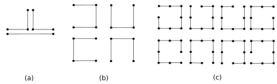
\includegraphics[width=12cm]{./img/b1epgSub.pdf}
\end{center}
\caption{Minimal non-Helly sub-families for the $B_1$, $B_2$ and $B_3$ -families.}
\label{fig:lowerBoundBkEPG1}
\end{figure}

Observe that for $k=4$ we can always to construct families $\cal{F}$ that are $(n-1)$-intersecting, while $core({\cal{F}})=\emptyset$ (see Figure~\ref{fig:lowerBoundB4EPG}). Therefore $H(B_4$-EPG) is unbounded. Clearly the same holds for $k >4$. 

\begin{figure}[!h]
\begin{center}
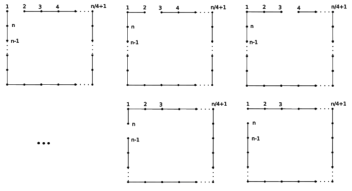
\includegraphics[width=12.5cm]{./img/b4epg.pdf}
\end{center}
\caption{$B_4$-EPG has an unlimited Helly number.}
\label{fig:lowerBoundB4EPG}
\end{figure}

Next, we consider upper bounds for the Helly number $B_k$-EPG graphs.

\subsection{Upper Bounds}\label{subsec-upper}

In order to obtain tight upper bounds for the Helly number, in terms of the number of bends, we introduce below more notation and lemmas.

Say that a set of edges of a grid is {\it co-linear} if all edges of the set belong to the same line of the grid, horizontal or vertical. The set of edges is called {\it parallel} if all its edges lie on parallel lines of the grid, but no two of them are co-linear.  


\begin{lemma}
\label{lemma:3colin}
Let $\cal {F}$ be a minimal non-$(h-1)$-Helly family of paths on a grid containing three co-linear non-representative edges. Then $\cal{F}$ must contain paths with at least four bends.
\end{lemma}



\begin{lemma}
\label{lemma:3par}
Let $\cal{F}$ be a minimal non-$(h-1)$-Helly family of paths on a grid, containing three parallel edges, and having  Helly number $H(\cal{F})$   $\geq 4$. Then $\cal{F}$ must contain paths with at least four bends. 
\end{lemma}


\begin{lemma} \label{lemma:Lwit}
Let $\cal{F}$ be a minimal non-$(h-1)$-Helly family of paths on a grid with  Helly number $H({\cal F}) \geq 4$. If ${\cal F}$ contains three non-representative edges that lie on a common $B_1$-subpath $P_i$, then $\cal {F}$ must have some path with at least three bends. \end{lemma}


The following are tight upper bounds for the Helly numbers of $B_k$-EPG paths, for $k = 1,2,3$.

\begin{claim}\label{claim:upper-B1}
$H(B_1$-$EPG) \leq 3.$
\end{claim}
 
\proof
Assume by contradiction that the Helly number of $B_1$-EPG paths is $h > 3$. In this case, consider a minimal non-$(h-1)$-Helly family of $\cal F$ of $B_1$-EPG paths. Then $\cal F$ contains at least $h$ paths.  
Any path $P_1 \in \cal{F}$ must contain $h-1$ non-representative edges  corresponding to the $h-1$ distinct paths of $\cal F$ other than $P_1$. Since $h-1 \geq 3$, $P_1$ contains at least three distinct non-representative edges $u_2, u_3, u_4 \in P_i$, with $u_3$ lying  between $u_2$ and $u_4$ in the path.   

If $u_2$, $u_3$ and $u_4$ are co-linear then by Lemma~\ref{lemma:3colin} $P_3 \in \cal{F}$ must contain at least four bends. Otherwise, the edges must lie on $P_1$ which has a single bend. Thus, it follows from Lemma~\ref{lemma:Lwit} that $P_3$ has three bends. In any situation, a contradiction arises, implying that $H({\cal F}) \leq 3$.
\qed

\begin{claim}\label{claim:upper-B2}
$H(B_2$-EPG$) \leq 4.$
\end{claim}

\proof
Assume by contradiction that the Helly number of  $B_2$-EPG families of paths is $h > 4$. Consider a minimal non-$(h-1)$-Helly family $\cal F$ of $B_2$-EPG paths. The family  $\cal F$ must contain at least $h \geq 5$ distinct paths, each of them corresponding to a distinct non-representative edge. Choose arbitrarily 5 of these non-representative edges.

By Lemmas ~\ref{lemma:3colin} and ~\ref{lemma:3par} any three of these chosen edges can  neither be co-linear nor parallel. Therefore, at least one of the five chosen non-representative edges must be in a different direction from the majority of the chosen edges. Call the direction of this edge vertical and the direction of the majority of the chosen edges horizontal. Consider a path $P_1$ from the family $\cal F$ that goes through this vertical edge. 
The path $P_1$ contains at least four of the chosen non-representative edges, at least one of which is vertical. Since $P_1$ has at most two bends, then it must have at most three segments. Since we have three segments and four non-representative edges which $P_1$ must contain, by the pigeon hole principle, one of these segments must have two non-representative edges. If this pair of edges are in a horizontal segment of $P_1$, then such pair of edges, along with the vertical edge are in two consecutive path segments, forming a $B_1$-subpath in $\cal F$. Then Lemma~\ref{lemma:Lwit} implies that some path of $\cal F$ must have at least three bends.   Otherwise, the two edges are vertical. But the others must be horizontal, and again we have at least three edges in a pair of consecutive segments forming a subpath in $\cal F$ having one bend. Again,  Lemma ~\ref{lemma:Lwit} implies that some path has at least three bends.
\qed

\begin{claim}\label{claim:upper-B3}
$H(B_3$-EPG$) \leq 8.$
\end{claim}

\proof
Assume by contradiction that the Helly number of  $B_3$-EPG paths is $h > 8$. In this case, consider a minimal non-$(h-1)$-Helly family $\cal F$ of $B_3$-EPG paths. Then $\cal F$ contains at least $h$  distinct non-representative edges,  corresponding to $h$ distinct paths.  By Lemma~\ref{lemma:3par}, since we can have at most three bends in any path, then these $h$  non-representative edges must lie in at most two vertical and two horizontal lines of the grid. Therefore one of these four possible lines must contain at least three distinct non-representative edges. By Lemma~\ref{lemma:3colin},  that would imply the existence of a path with four bends.\qed

This completes the proof of Theorem \ref{thm:Helly-EPG}. 


\section{Helly number of $B_k$-VPG Graphs}\label{sec:HellynumberVPG}

In this section, we determine the Helly number of $B_k$-VPG graphs. We prove the following results.
\begin{theorem}\label{thm:Bk-VPG}
The Helly numbers for $B_k$-VPG graphs satisfy:
\begin{enumerate}
\item $H(B_1$-VPG) = 4.
\item $H(B_2$-VPG) = 6.
\item $H(B_3$-VPG) = 12.
\item $H(B_4$-VPG) is unbounded.
\end{enumerate}
\end{theorem}

Again, we prove the theorem by showing tight lower and upper bounds.

\subsection{Lower Bounds}

%First, we describe lower bounds.
We start by describing some sets of paths that achieve our lower bounds. 
Figure \ref{VPG:lower-B1} shows a set of 4 $B_1$-paths of a graph $G$, in a $2 \times 2$ grid, such that each path covers three vertices of the grid, and avoids exactly one of the vertices. 

\begin{figure}[!h]
    \centering
    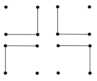
\includegraphics[width=3cm]{./img/lower-bound-B1-VPG.pdf}
    \caption{Lower bound for $B_1$-VPG graphs.}
    \label{VPG:lower-B1}
\end{figure}

Figure \ref{VPG:lower-B2} shows a set of 6 $B_2$-paths of a graph $G$, in a $2 \times 3$ grid, such that each path covers five vertices of the grid, and avoids exactly one. 


\begin{figure}[!h]
    \centering
    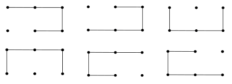
\includegraphics[width=8cm]{./img/lower-bound-B2-VPG.pdf}
    \caption{Lower bound for $B_2$-$VPG$ graphs.}
    \label{VPG:lower-B2}
\end{figure}


Figure \ref{VPG:lower-B3} shows 12 $B_3$-paths of a graph $G$, in a grid, of perimeter 12, such that each path covers 11  vertices of the grid,  avoiding one of them. 

\begin{figure}[!h]
    \centering
    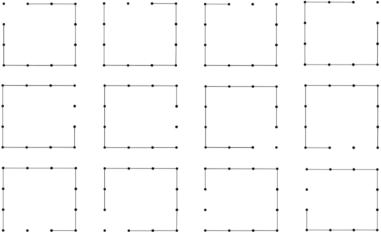
\includegraphics[width=12cm]{./img/lower-bound-B3-VPG.pdf}
    \caption{Lower bound for $B_3$-VPG graphs.}
    \label{VPG:lower-B3}
\end{figure}

Figure \ref{VPG:lower-B4} shows a set of $n$ $B_4$-paths of a $n$-vertex graph $G$, in a grid having perimeter $n$,  such that each path covers $n-1$  vertices of $G$, avoiding one of them. 

\begin{figure}[!h]
    \centering
    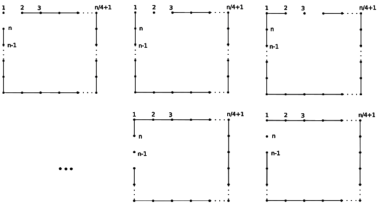
\includegraphics[width=12cm]{./img/lower-bound-B4-VPG.pdf}
    \caption{Lower bound for $B_4$-VPG graphs.}
    \label{VPG:lower-B4}
\end{figure}

Applying Theorem \ref{thm:minimal}, we can then conclude that the number of vertices of each of the above-described graphs is lower bound for the corresponding class. Then, we can claim the following bounds.

\begin{claim}\label{claim:VPG-lower}
The following are lower bounds for the Helly numbers of $B_k$-VPG graphs.
\begin{enumerate}
\item $H(B_1$-VPG) $\geq 4$.
\item $H(B_2$-VPG) $\geq 6$.
\item $H(B_3$-VPG) $\geq 12$.
\item $H(B_4$-VPG) is unbounded.
\end{enumerate}
\end{claim}

\subsection{Upper Bounds}

Next, we provide upper bounds for the Helly number of $B_k$-VPG graphs. The following lemmas are employed.

\begin{lemma}\label{column-sizes}
Let $\cal F$ be a minimal non-$(h-1)$-Helly family of paths, for some $h$, containing $k \in \{3,4,5\}$ distinct co-linear non-representative points of the grid. Then $\cal F$ contains a path having at least $k-1$ bends.
\end{lemma}

% \proof For $k \in \{3,5\}$, the path avoiding the middle point has at least $k-1$ bends, while for $k = 4$, the path avoiding one of the middle points also has this same property.
% \qed

\begin{lemma}\label{column-number}
Let $\cal F$ be a minimal non-$(h-1)$-Helly family of paths, on a grid containing $k < h$ distinct pairwise non-co-linear non-representative points. Then $\cal F$ must contain a path with at least $k-1$ bends.
\end{lemma}   

% \proof Since $k < h$, $\cal F$ must contain a path that visits all such $k$ pairwise non-co-linear points. Such a path requires at least one bend, between two consecutive non-co-linear points. Therefore $\cal F$ contains a path with at least $k-1$ bends. \qed \\

We also employ some additional concepts and notation, below described.

Let $\cal F$ be a minimal non-$(h-1)$-Helly family of $B_{k-1}$-paths on a grid $Q$. By Theorem \ref{thm:minimal},  we can choose $h$ paths $P_i \in {\cal F}$, each of them associated to a distinct non-representative grid point $p_i$, such that $P_i$ avoids $p_i$, but contains all the other $h-1$ distinct non-representative points $p_j \in P_J$, for each   $j \neq i$. Denote by $P_N$, $|P_N|=h$, the subset of grid  points of  $Q$, restricted to the chosen set of distinct  non-representative points $p_i$. By Lemmas \ref{column-sizes} and \ref{column-number}, the grid points of $P_N$ are contained in at most $k$ columns (lines), and each column (line) contains at most $k$ points of $P_N$. Consequently, the cardinalities of the points of $P_N$, contained in the columns (lines) of $Q$,  form a partition of the integer $h$, into at most $k$ parts, such that each part is at most $k$. Call such a partition as a {\it feasible  partition  of $h$, relative to $P_N$}. Therefore, each non-representative point $p_i \in P_N$ contributes with one unit to some part of the partition, which is then referred to,   as the part of the partition {\it corresponding} to $p_i$.    

The following lemma describes sufficient conditions for an integer $h$ to be an upper bound for the Helly number.

\begin{lemma}\label{upper-bound} Let $\cal F$ be a minimal non-$(h-1)$-Helly family of $B_{k-1}$-paths on a grid $Q$, and $P_N$ the set of non-representative points of $Q$. Let $k,h$ be integers, $1 \leq k \leq 3$ and $k < h$. The following conditions imply $H(B_k$-VPG) $\leq h$  
\begin{itemize}
    \item[(i)] there is no feasible partition of $h+1$, relative to $P_N$, or 
    \item[(ii)] for any possible feasible partition, and for any arrangement of the grid points of $P_N$ in $Q$, there is some non-representative point $p_i \in P_N$, such that  no path exists  in $Q$, having at most $k$ bends, containing all points of $P_N$, except $p_i$.    
\end{itemize}
\end{lemma}
{\it Proof}: The proof of (i) follows from Lemmas \ref{column-sizes} and \ref{column-number}, while the proof of (ii) is a consequence of Theorem \ref{thm:minimal}.  \qed \\

The following are upper bounds for the Helly number of $B_k$-VPG graphs, for each $k$, $1 \leq k \leq 3$, obtained  by applying Lemma \ref{upper-bound}.      
 
\begin{claim}\label{claim:upper-B1-VPG}
$H(B_1$-VPG) $\leq  4$.
\end{claim}

% \proof There is no partition of the integer 5, into two parts, in which each part is at most 2. Consequently, the result follows from Lemma \ref{upper-bound} (i). \qed

\begin{claim}\label{claim:upper-B2-VPG}
$H(B_2$-VPG)  $\leq  6$.
\end{claim}

% \proof Assume the contrary. Then $H(B_2$-VPG) $\geq  7$, let $\cal F$ be a minimal non-6-Helly family of $B_2$-paths, and  $P_N$ be the set of non-representative points of $\cal F$ in $Q$. There are two possible partitions of the integer 7, in three parts, each of them of size at most 3, namely $(3,3,1)$ and $(3,2,2)$. In any of these cases,  it is always possible to choose some point  $p_i \in P_N$, belonging to a part of the partition of size 3, such that a path in $\cal F$  which avoids $p_i$ and covers the other six non-representative points, must contain at least three bends.  Then by Lemma \ref{upper-bound}, indeed $H(B_2$-VPG)  $\leq  6$. \qed


\begin{claim}\label{claim:upper-B3-VPG}
$H(B_3$-VPG) $\leq  12$.
\end{claim}

% \proof Assume the contrary, $H(B_3$-VPG) $\geq  12$. Let $\cal F$ be a minimal non-12-Helly family of $B_3$-paths, and  $P_N$ be the set of non-representative points of $\cal F$ in $Q$. There are three possible partitions of the integer 13, into four parts, each of them of size at most 4, namely $(4,4,4,1)$, $(4,4,3,2)$ and $(4,3,3,3)$. In this case, choose $p_i \in P_N$ to be a non-representative point, corresponding to a part of size $4$ of the partition.  The path of ${\cal F}$, which avoids $p_i$, must cover the other 12 non-representative points. These points are located in 4 distinct columns, of cardinalities 4,4,3,1, 4,3,3,2, or 3,3,3,3, considering the three possible partitions, respectively. Such a path must contain at least four bends, a contradiction. Then by Lemma \ref{upper-bound}, $H(B_3$-VPG) $\leq  12$.    \qed  

From the lower and upper bounds described in the previous subsections, we obtain the results for the Helly numbers of $B_k$-VPG graphs, completing the proof of Theorem \ref{thm:Bk-VPG}.

\section{Strong Helly Number} \label{sec:strongHellyNumber}

In this section, we first consider determining the strong Helly number of $B_k$-EPG graphs.

We start by describing a theorem similar to Theorem \ref{thm:minimal}.

\begin{theorem}\label{thm:minimal-strong}

Let ${\cal C}$ be a hereditary class of families $\cal F$ of subsets of the universal set $U$, whose strong Helly number $sH({\cal C})$ equals $h$. Then there exists a family ${\cal F'} \in {\cal C}$ with exactly $h$ subsets satisfying the following condition: 

For each subset $P_i \in \cal {F'}$, there is exactly one distinct element $u_i \in U$, such that \\
$$u_i \not \in P_i,$$ 
but $u_i$ is contained in all  subsets 
$$P_j \in {\cal F'} \setminus P_i.$$
\end{theorem}

Proof: The strong Helly number of ${\cal C}$ is $h$ and not $h - 1$, so that  there must exist some family ${\cal F} \in {\cal C}$ whose strong Helly number is exactly $h$, i.e., $\cal F$  contains $h$ subsets $P_i$ whose intersection equals  core($\cal F'$) but is such that no  $h-1$ of its subsets have the same intersection. In particular, let $\cal F'$ be the family containing exactly the $h$ subsets $P_i$ described above. Such a family must exist, since $\cal C$ is hereditary. Then each $P_i$ does not contain at least one element $u_i$ in the intersection of the remaining $h-1$ subsets $P_j$, $j \ne i$, 
since the intersection of these $h-1$ subsets must not be equal to the core($\cal F'$).  \qed

Again, if we consider the family $\cal F'$ described in the theorem above it is simple to conclude that the removal of any subset from $\cal {F'}$ turns it $(h-1)$-strong Helly.  Then call $\cal {F'}$ a {\it minimal} non-$(h-1)$-strong Helly family. Moreover, the element $u_i \not \in P_i$, contained in all subsets $P_j \in {\cal{F'}} \setminus P_i$, except $P_i$, is the {\it $h$ non-representative} of $P_i$.  

As before, we employ the above minimal families of subsets, applied to paths in a grid.

We prove that the strong Helly number of $B_k$-EPG graphs coincide with the Helly number, for each corresponding value of $k$. Similarly, for $B_k$-VPG graphs. For $k=0$, it is simple to show that if a set of intervals $\cal I$ in a line pairwise intersect, then there exist two intervals of $\cal I$, whose intersection equals the intersection of all intervals of $\cal I$. Consequently, the $k$-strong Helly number of $B_0$-EPG graphs equals 2. 
Similarly, for $B_0$-VPG graphs. 
Recall that the strong Helly number is at least equal to the Helly number of a family so that the lower bounds presented in Claim~\ref{claim:lower-Bk-EPG} also hold for the strong Helly number. The proofs for the strong Helly numbers for $k \geq 1$ are similar to those described in Section \ref{sec:Helly-number}.  



\section{Concluding Remarks}\label{sec:concludingRemarks}
We have determined the Helly number and strong Helly number of $B_k$-EPG graphs and $B_k$-VPG graphs, for $k \geq 0$. 

Table \ref{tab:Helly-Strong-Helly} summarizes the results obtained.
 
\Large 

\begin{table}[htb]
    \centering
    \caption{Helly and Strong Helly Numbers for $B_k$-EPG and $B_k$-VPG Graphs}
    \label{tab:Helly-Strong-Helly}
    \begin{tabular}{c|c|c}
     \multicolumn{3}{c}{}\\
    \cline{1-3} $k$  & $B_k$-EPG & $B_k$-VPG \\
    \cline{1-3} 0 & 2 & 2 \\
    \cline{1-3} 1 & 3 & 4 \\
    \cline{1-3} 2 & 4 & 6 \\
    \cline{1-3} 3 & 8 & 12 \\
    \cline{1-3} $\geq 4$ & unbounded & unbounded \\
    \cline{1-3} 
    \end{tabular}
\end{table}

\normalsize

We leave two questions to be investigated concerning the presented results.

\begin{enumerate}
\item Given a {\it specific}  EPG or VPG graph, the question is to formulate an algorithm to determine its Helly and strong Helly numbers. See \cite{dourado2008improved}, for instance, for such algorithms, applied to general graphs. 

\item The values of the Helly and strong Helly numbers, which were determined in this chapter, coincided in all cases. Clearly, in general, this is not the case. We leave as an open question, to find the conditions for such equality to occur. \end{enumerate}


\newpage


\section{Article submitted to journal  Discussiones Mathematicae Graph Theory (DMGT)} 
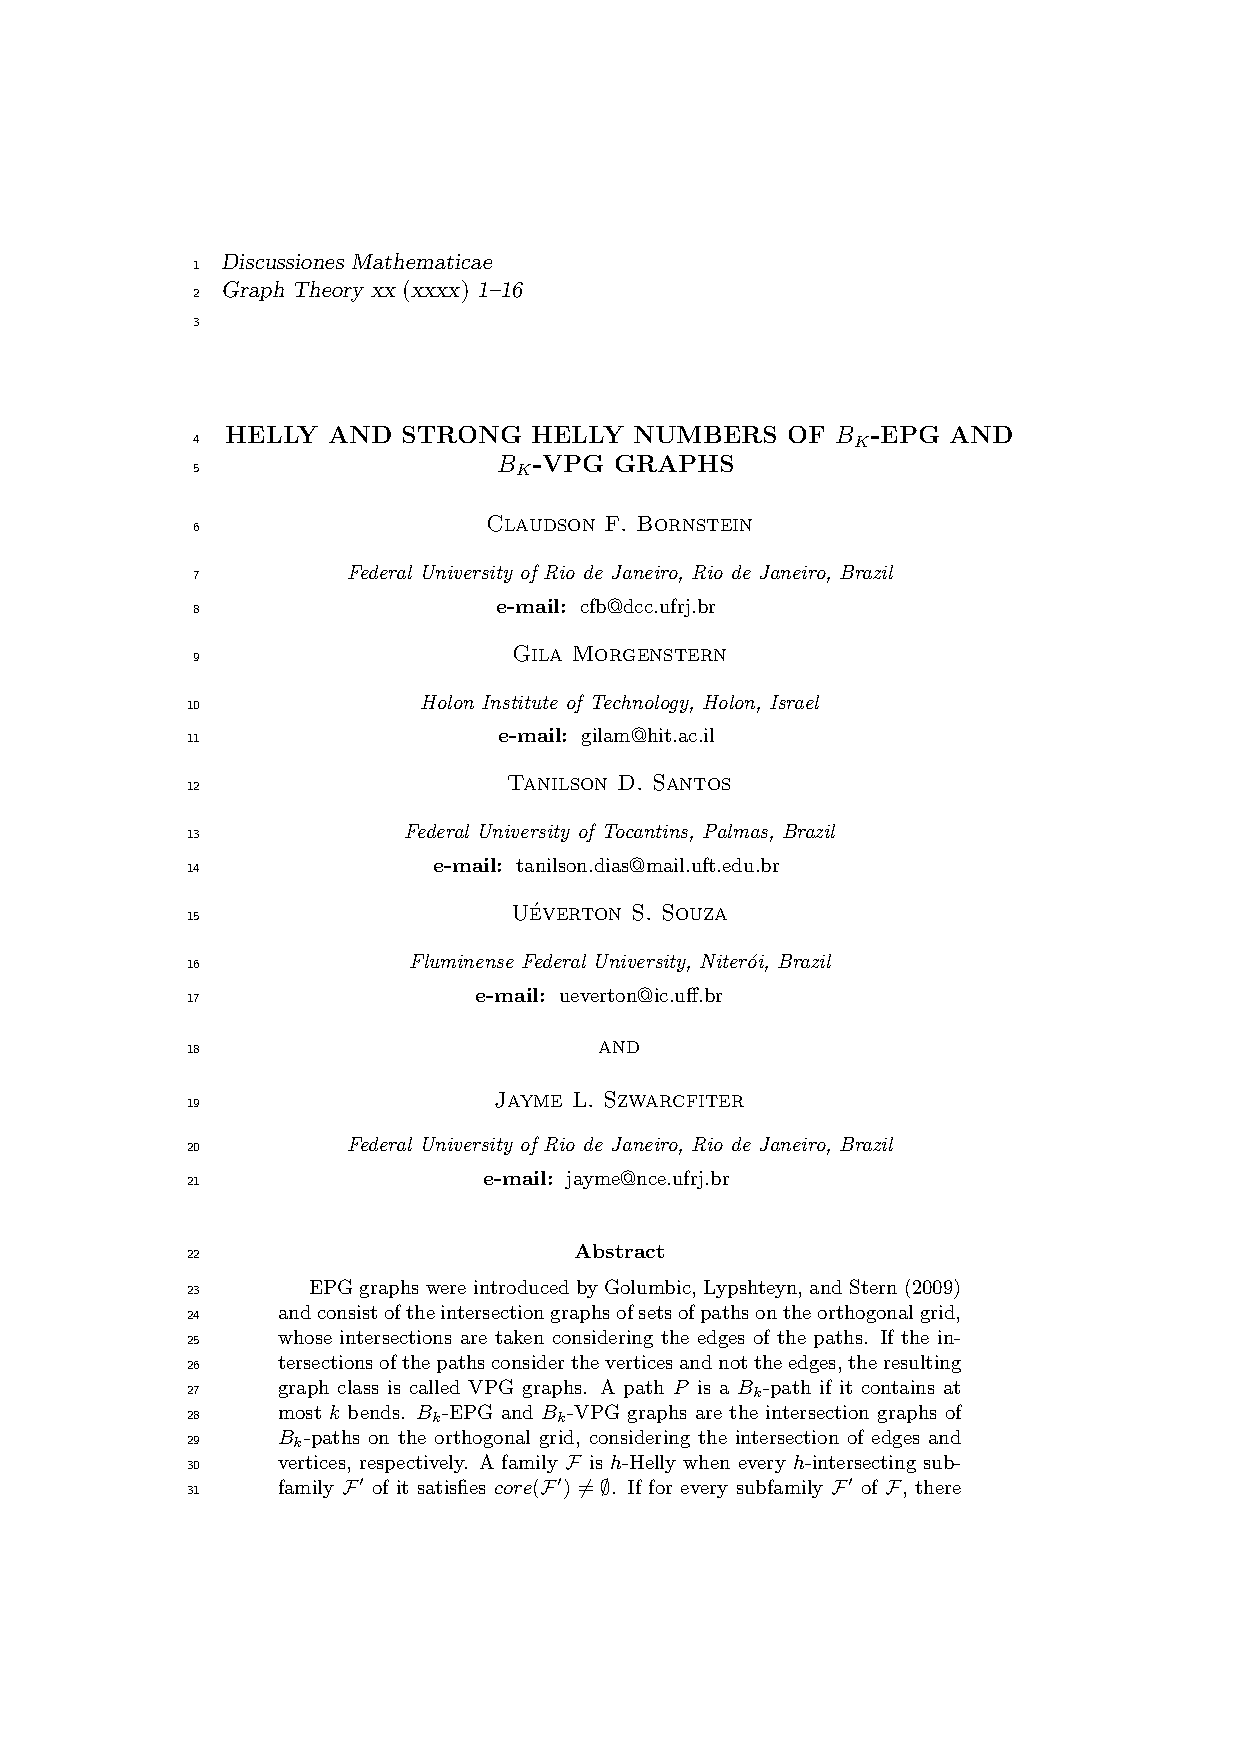
\includepdf[pages=-]{./includes/include-pdf-files/paperDMGT2020.pdf}